\chapter{Omologia}


\section{Omotopie e retratti}

\begin{definition}
	Siano $\morphism{f_0, f_1}{X}{Y}$ mappe continue. Allora $f_0$ e $f_1$ si dicono \textbf{omotope} se esiste una funzione continua $\morphism{F}{X \times \left[0,1\right]}{Y}$ tale che $F(t,0) = f_0(t)$ per ogni $t \in X$ e $F(t,1) = f_1(t)$ per ogni $t \in X$.
\end{definition}

\begin{remark}
	L'omotopia è una relazione di equivalenza. 
\end{remark}

\begin{definition}
	Siano $\morphism{f_0, f_1}{X}{Y}$ mappe continue e sia $A \subset X$. Allora $f_0$ e $f_1$ si dicono \textbf{omotope relativamente ad} $A$ se esiste una funzione continua $\morphism{F}{X \times \left[0,1\right]}{Y}$ tale che $F(t,0) = f_0(t)$ per ogni $t \in X$ e $F(t,1) = f_1(t)$ per ogni $t \in X$ e $F(a, t) = f_0(a) = f_1(a)$ per ogni $a \in A$.
\end{definition}

\begin{definition}
	Due spazi topologici $X,Y$ si dicono \textbf{omotopicamente equivalenti} se esistono le mappe continue $\morphism{f}{X}{Y}$,$\morphism{g}{Y}{X}$ tali che $g \circ f \sim \idarrow[X]$ e $f \circ g \sim \idarrow[Y]$. 
\end{definition}

\begin{remark}
	L'omotopia di spazi topologici è una relazione di equivalenza. 
\end{remark}

\begin{definition}
	Se $A \subset X$ dove $X$ spazio topologico allora $A$ è detto \textbf{retratto} di $X$ se esiste $\morphism{r}{X}{A}$ con $r$ continua e che $r(a) = a$ per ogni $a \in A$. In particolare $r \circ i_A = \idarrow[A]$.
\end{definition}

\begin{definition}
	$A$ è detto \textbf{retratto di deformazione} di $X$ se è un ritratto e $i_A \circ r \sim \idarrow[X]$.
\end{definition}


\begin{remark}
	Alcuni esempi
	\begin{enumerate}
		\item Dimostriamo che $\R^n \setminus \{0\} \sim \Circ^{n-1}$ definiamo come retratto $\morphism{r}{\R^n \setminus \{0\}}{\Circ^{n-1}}$ con $r(x) = \frac{x}{\|x\|}$. Allora è ovvio che $r \circ i = \idarrow[\Circ^{n-1}]$. Prendiamo quindi il caso $i \circ r = \frac{x}{\|x\|}$ con $x \in \R^n  \setminus \{0\}$. Dimostriamo che questa funzione è omotopa all'identità su $\R^n \setminus \{0\}$. Usiamo l'omotopia $F(s,t) = (1-t)(i \circ r) + tx$ e abbiamo concluso.
		\item Definiamo ora la somma topologica di due spazi topologici $(X, \tau_1), (Y, \tau_2)$ disigunti. L'unione verrà definita come $(X \cup Y, \tau)$ dove $\tau$ è la topologia i cui aperti sono tali per cui $A \in \tau$ allora $A \cap X \in \tau_1$ e $A \cap Y \in \tau_2$. Mentre la somma topologica vera e propria $X \lor Y$ è definita come $X \lor Y := (X \cup Y, \tau) / \sim_{a_0, b_0}$ dove $ a \sim_{a_0, b_0} b \leftrightarrow a = b \lor (a = a_0 \land b = b_0)$. Ovvero unisce gli spazi e fa coincidere un punto dei rispettivi nello stesso. In pratica consideriamo il bouquet di due circonferenze $\Circ^1 \lor \Circ^1$ rappresentato in figura.
		
		\begin{figure}[h]
			\centering
			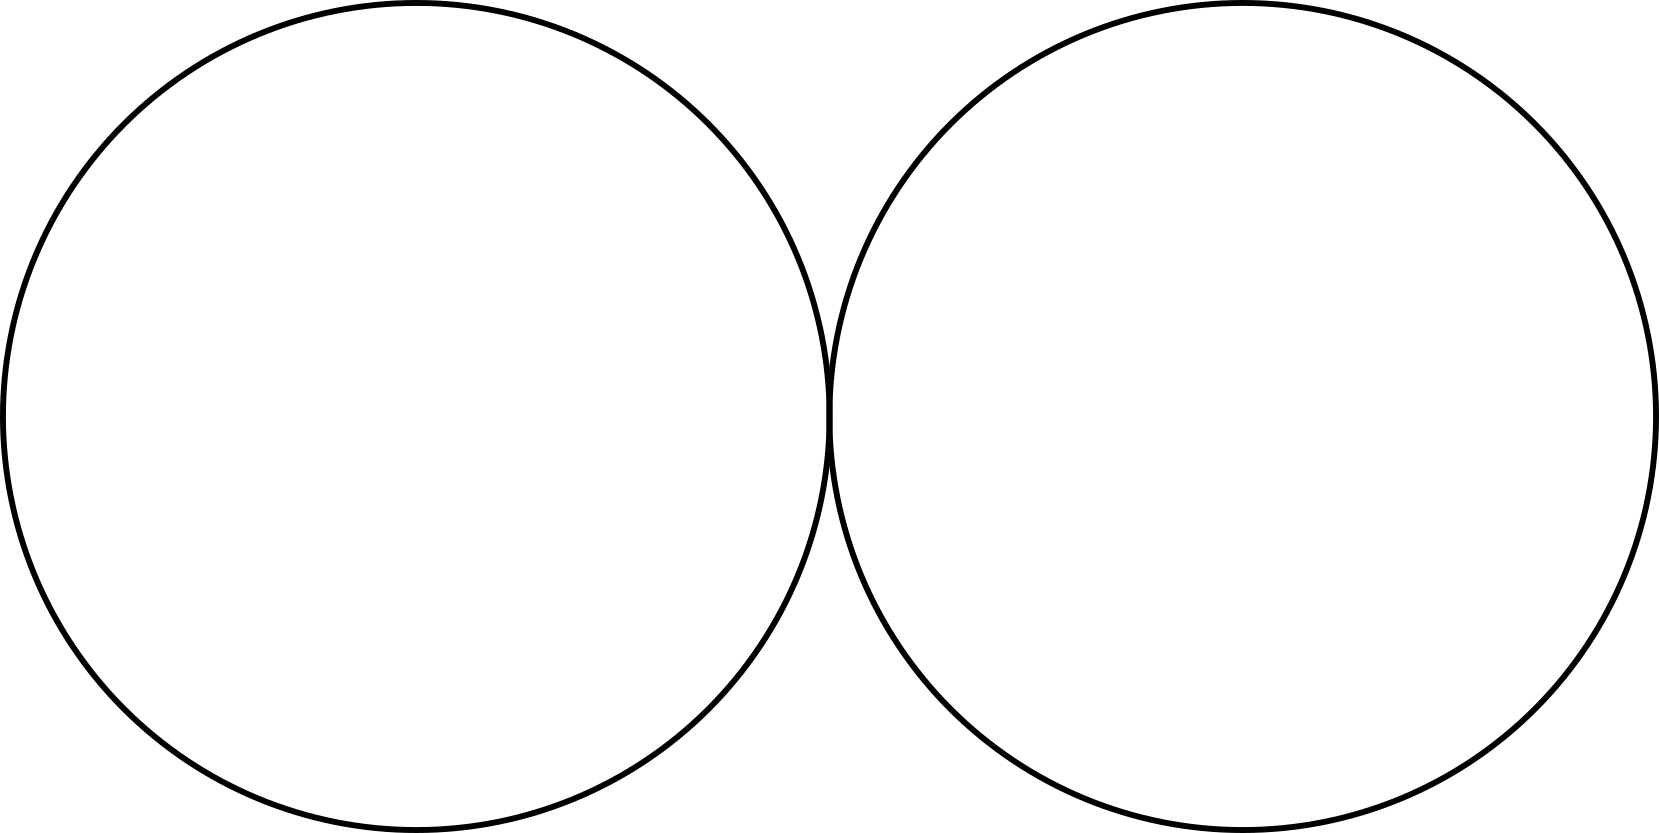
\includegraphics[width=0.3\linewidth]{images/bouquet_circonferenze}
			\caption{}
			\label{fig:bouquetcirconferenze}
		\end{figure}
		Questo è ovviamente omotopo a $\R^2 \setminus \{(-1,0), (1,0)\}$ dove i punti scelti possono essere presi secondo propria volontà.
		\item Se $X \subset \R^n$ ed è un sottospazio stellato rispetto al centro $x_0$ allora $Y = \{x_0\}$ è un retratto di $X$. Infatti $X \sim \{p\}$ per qualsiasi $p \in \R^n$. Mostriamo intanto che $Y \sim X$. L'omotopia $F(x,t) = x - t(x-x_0)$ porta, in modo continuo, dalla funzione di $\morphism{id}{X}{X}$ (ovvero $x \mapsto x$) a $\morphism{i}{X}{X}$ (ovvero $x \mapsto x_0$). Ovvero $Y \sim X$.
		\item Sia $X = T$ toro. Allora $\morphism{r}{T}{\Circ^1}$ è un retratto su $\Circ^1 \subset T$, ma non è un retratto di deformazione. Infatti è impossibile trasformare (in modo continuo) un toro in una circonferenza. 
		\item Se si toglie un punto a il $g$-toro allora $T_g \setminus \{t\} \sim \underbrace{\Circ^1 \wedge \dots \wedge \Circ^1}_{2g-\text{volte}}$ e analogamente per il piano proiettivo $U_h$ senza un suo punto $U_h \setminus \{p\} \sim \underbrace{\Circ^1 \wedge \dots \wedge \Circ^1}_{h-\text{volte}}$
 	\end{enumerate}
\end{remark}

\section{CW-complessi}

Ora verranno introdotte delle classi di insiemi tali che possono essere suddivisi in parti \textit{retratte} e parti irriducibilmente non retratte, ovvero il Teorema \ref{thr:contrai_ncelle_cw_complesso}.

\begin{definition}
	Uno spazio topologico $X$ si dice n-\textbf{cella} se $X \simeq \D^n$.
\end{definition}

\begin{definition}[Procedura di incollamento]
	\label{def:incollamento}
	L'incollamento di due spazi topologici $X,Y$ tramite $A \subset X$ è rapprensentato dal seguente diagramma
	\begin{equation}
	\begin{tikzcd}
	A \arrow[d, hook]{i} \arrow[r]{f} & Y \\
	X
	\end{tikzcd}
	\end{equation} 
	lo spazio topologico risultante dall'incollamento è $X \sqcup Y / \sim$ dove $x \sim y \in Y \Longleftrightarrow x \in A \land f(x) = y$.
\end{definition}

\begin{definition}[Algoritmo di costruzione di un CW-complesso finito]
	$X$ è un CW-complesso se è possibile costruirlo secondo il seguente algoritmo:
	\begin{enumerate}
		\item Dato $X^0 \neq \varnothing$ insieme finito (detto anche $0$-scheletro)
		\item Sia $n \ge 1$ allora per ipotesi induttiva supponiamo $X^{n-1}$ $(n-1)$-scheletro come ipotesi. Allora si incollano a $X^{n-1}$ delle $n$-celle attraverso il procedimento della Definizione \ref{def:incollamento} in cui vale 
		\begin{equation}
		\begin{tikzcd}
			\Circ^{n-1} = \partial \D^n \arrow[d, hook]{i} \arrow[r]{f} & X^{n-1} \\
			\D^n
		\end{tikzcd}
		\end{equation} 
		con $X^n = X^{n-1} \sqcup \D^n / \sim$ con la relazione specificata nella procedura di incollamento.
		\item Se il CW-complesso è di dimensione $N$, allora per $n = N$ il procedimento termina, con $X^N = X$.  
	\end{enumerate}
\end{definition}

\begin{definition}
	Sia $X$ un CW-complesso allora una n-cella chiusa in $X$ è l'immagine di $\morphism{f}{\D^n}{X}$ dove $f$ è definita come nella seguente successione
	\begin{equation}
	\begin{tikzcd}
		\D^n \arrow[bend right=25, swap, hook]{rr}{f} \arrow[r,hook] & \D^n \sqcup X^{n-1} / \sim \arrow[r,hook] & X
	\end{tikzcd}
	\end{equation}
\end{definition}

\begin{remark}
	In generale $\image{f} \neq \D^n$. Per esempio si prenda la costruzione di $\Circ^2$ come un CW-complesso con una $0$-cella e una $2$-cella che identifica tutto il suo bordo nel punto. Allora 
	\begin{equation}
	\begin{tikzcd}
		\D^2 \arrow[bend right=25, swap, hook]{rr}{f} \arrow[r,hook] & \D^2 \sqcup \{p\} / \sim \arrow[r,hook] & \Circ^2
	\end{tikzcd}
	\end{equation}
	è ovvio che $\image{f} = \Circ^2 \neq \D^2$. 
\end{remark}

\begin{definition}
	Sia $X$ un CW-complesso allora una n-cella aperta in $X$ è l'immagine di $\morphism{f}{\D^n}{X}$ dove $f$ è definita come nella seguente successione
	\begin{equation}
	\begin{tikzcd}
	\mathring{\D}^n \arrow[bend right=25, swap, hook]{rr}{f} \arrow[r,hook] & \mathring{\D}^n \sqcup X^{n-1} / \sim \arrow[r,hook] & X
	\end{tikzcd}
	\end{equation}
\end{definition}

\begin{remark}
	Le $n$-celle aperte sono omeomorfe al disco aperto $\mathring{\D}^n$. Infatti 
	\begin{equation}
		\mathring{\D}^n \sqcup X^{n-1} / \sim\ = \mathring{\D}^n \sqcup X^{n-1}
	\end{equation}
	poiché il bordo non dev'essere identificato (non fa parte dell'insieme $\mathring{\D}^n$).
\end{remark}

\begin{theorem}
	\label{thr:contrai_ncelle_cw_complesso}
	Se $X$ è un CW-complesso e $A \subset X$ è un sottocomplesso chiuso (ovvero un unione di $n$-celle chiuse) vale che se $A$ è contraibile allora $X$ è omotopo a $X / A$.
\end{theorem}
\begin{proof}
	% TODO 
\end{proof}

I CW-complessi sono importanti poiché è possibile esprimere un invariante topologico. Infatti se due CW-complessi sono omeomorfi allora il valore della funzione caratteristica di Eulero è uguale. 

\begin{definition}
	Sia $X$ un CW-complesso costituito da $n_0$ $0$-celle, $\dots$, $n_N$ $N$-celle, allora 
	\begin{equation}
	\begin{aligned}
		\chi(X) = \sum_{i=0}^{N} (-1)^i n_i
	\end{aligned}
	\end{equation}
	è il numero della funzione caratteristica di Eulero di $X$. 
\end{definition}

\begin{remark}
	Alcuni esempi di CW-complessi
	\begin{enumerate}
		\item In generale un $g$-toro è composto da $1$ $0$-cella, $2g$ $1$-celle, $1$ $2$-cella. Quindi ha numero caratteristico $\chi(T_g) = 2(1-g)$. 
		\item In generale un piano proiettivo $U_h$ è composto da $1$ $0$-cella, $h$ $1$-celle, $1$ $2$-cella. Quindi ha numero caratteristico $\chi(U_h) = 2 - h$.
		\item Il disco $\D^n$ è una $n$-cella quindi $\chi(\D^n) = (-1)^n$. In generale il disco $n$-esimo si può costruire con una $0$-cella, una $(n-1)$-cella e $1$ $n$-cella.
	\end{enumerate}
\end{remark}

\begin{remark}
	Alcuni esempi del Teorema \ref{thr:contrai_ncelle_cw_complesso} possono essere i seguenti
	\begin{enumerate}
		\item Sia $X \subset \R^2$ come in figura 
		\begin{figure}[h]
			\centering
			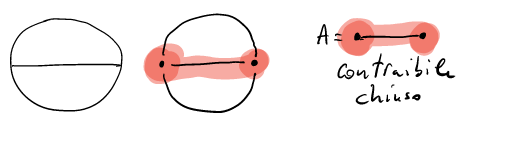
\includegraphics[width=0.6\linewidth]{images/CWCOMPLEXEsempio1}
			\caption{}
			\label{fig:cwcomplexesempio1}
		\end{figure}
		allora è omotopicamente equivalente a un buquet di due circonferenze se si identifica la $1$-cella del diametro in un punto da cui
		\begin{figure}[h]
			\centering
			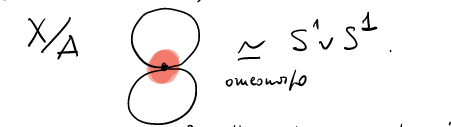
\includegraphics[width=0.6\linewidth]{images/CWCOMPLEXEsempio2}
			\caption{}
			\label{fig:cwcomplexesempio2}
		\end{figure}
		\item Sia $X \subset \R^2$ come in figura 
			\begin{figure}[h]
				\centering
				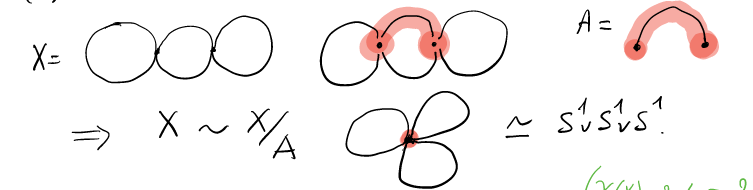
\includegraphics[width=0.7\linewidth]{images/CWCOMPLEXEsempio3.png}
				\caption{}
				\label{fig:cwcomplexesempio3}
			\end{figure}
			identifichiamo una 1-cella della circonferenza centrale (l'insieme $A$) in un punto così da ottenere un bouquet di $3$ circonferenze per il Teorema \ref{thr:contrai_ncelle_cw_complesso}.   
		\item Sempre come in figura è abbastanza esplicito  che il grafo sia omotopo a un buquet di $4$ circonferenze.
			\begin{figure}[h]
				\centering
				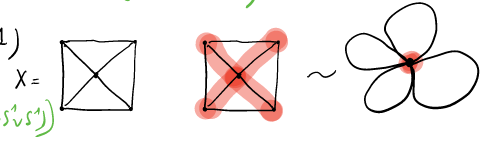
\includegraphics[width=0.7\linewidth]{images/CWCOMPLEXEsempio8.png}
				\caption{}
				\label{fig:cwcomplexesempi4}
			\end{figure}
		\item Sia $X$ un toro con un disco e una circonferenza 
			\begin{figure}[h!]
				\centering
				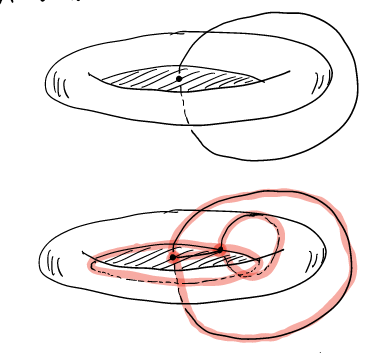
\includegraphics[width=0.3\linewidth]{images/CWCOMPLEXEsempi4}
				\caption{}
				\label{fig:cwcomplexesempi4}
			\end{figure}
			Allora $X$ è un CW-complesso composto da $2$ $0$-celle, $4$ $1$-celle, $2$ $2$-celle. Contriamo il disco al centro del toro in un punto (perché possiamo è un retratto).   
			\begin{figure}[h!]
				\centering
				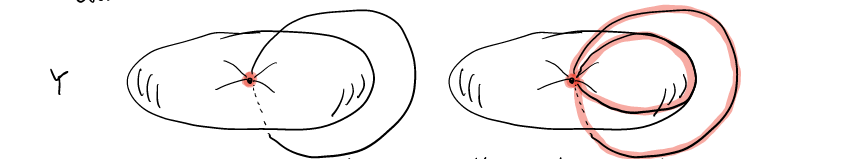
\includegraphics[width=0.7\linewidth]{images/CWCOMPLEXEsempi5}
				\caption{}
				\label{fig:cwcomplexesempi4}
			\end{figure}
			Indichiamo con $Y$ l'insieme con il disco retratto in un punto. Poi \textit{allarghiamo} il toro in modo tale da ottenere una sfera con dentro parte della circonferenza identificata, otteniamo uno spazio omotopo allo spazio $Z$ come in figura
			\begin{figure}[h!]
				\centering
				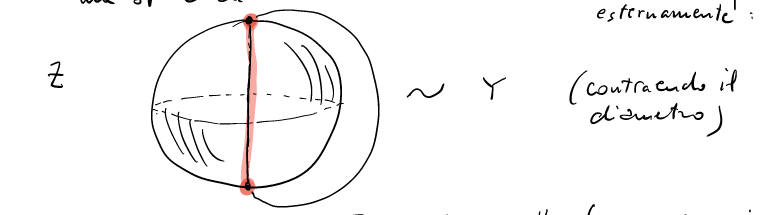
\includegraphics[width=0.7\linewidth]{images/CWCOMPLEXEsempi6}
				\caption{}
				\label{fig:cwcomplexesempi4}
			\end{figure}
			e studiando $Z$ si ottiene uno spazio omotopicamente equivalente a $\Circ^2 \lor \Circ^1 \lor \Circ^1$
			\begin{figure}[h!]
				\centering
				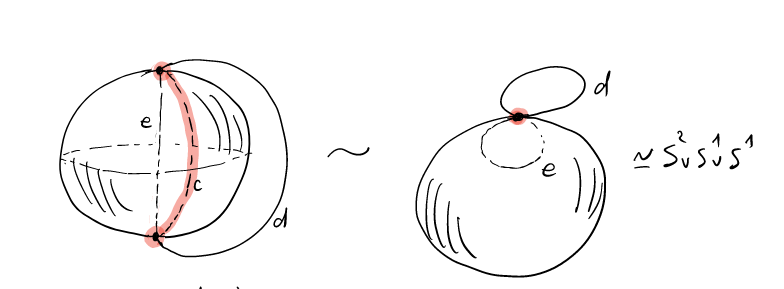
\includegraphics[width=0.7\linewidth]{images/CWCOMPLEXEsempi7}
				\caption{}
				\label{fig:cwcomplexesempi4}
			\end{figure}
			
	\end{enumerate}
\end{remark}

\section{Gruppo fondamentale}

\begin{definition}
	Sia $X$ spazio topologico, allora $\morphism{\alpha}{\left[0,1\right]}{X}$ tale che $\alpha(0) = x_0 \in X$ e $\alpha(1) = x_0 \in X$ con $\alpha$ continua si dice \textbf{cappio}.
\end{definition}

\begin{definition}
	Uno spazio topologico $X$ si dice semplicemente connesso se $\pi_1(X, x_0) \simeq (\{1\}, +)$ ovvero il gruppo banale. 
 \end{definition}

\begin{definition}
	Definiamo l'operatore $*$ come la composizione delle classi omotopiche di cappi $\alpha, \beta$ (aventi estremi congiungibili) come segue
	\begin{equation}
	\alpha * \beta :=
	\begin{cases}
		\alpha(2s) \quad 0 \le s \le 1/2 \\
		\beta(2s - 1) \quad 1/2 < s \le 1 \\ 
	\end{cases}
	\end{equation}
\end{definition}

\begin{theorem}
	Siano $\alpha, \beta$ due cammini in $X$ tali che sia definito il prodotto e analogamente per i cammini $\gamma, \delta$. Allora se $\alpha \sim \gamma$ e $\beta \sim \delta$ vale $\alpha * \beta \sim \gamma * \delta$
\end{theorem}
\begin{proof}
\end{proof}

\begin{theorem}
	$(\pi_1(X, x_0), *)$ forma un gruppo. In particolare valgono
	\begin{enumerate}
		\item $x_0 * \alpha \sim \alpha \sim \alpha * x_0$
		\item $\alpha * \overline{\alpha} \sim x_0 \sim \overline{\alpha} * \alpha$.
		\item $(\alpha * \beta) * \gamma \sim \alpha * (\beta * \gamma)$
	\end{enumerate} 
\end{theorem}
\begin{proof}
\end{proof}

\begin{theorem}
	Sia $X$ spazio topologico tale che $x_0 \in X$ è connesso per archi ad $x_1 \in X$, allora $\pi_1(X, x_0) \simeq \pi_1(X, x_1)$
\end{theorem}
\begin{proof}
	
\end{proof}

\begin{corollary}
	Se $X$ è connesso per archi allora il suo gruppo fondamentale è unico al più per isomorfismi.
\end{corollary}
	
	
\begin{theorem}
	Sia $\morphism{\varphi}{X}{Y}$ una mappa continua tra spazi topologici, allora induce un omomorfismo tra i relativi gruppi fondamentali $\morphism{\varphi_*}{\pi_1(X, x_0)}{\pi_1(Y, \varphi(x_0))}$. Inoltre l'operatore $_*$ ha proprietà funtoriali:
	\begin{enumerate}
		\item $(\varphi \circ \psi)_* = \varphi_* \circ \psi_*$
		\item $(\idarrow[X])_* = \idarrow[\pi_1(X, x_0)]$ 
	\end{enumerate}
\end{theorem}
\begin{proof}
\end{proof}

\begin{corollary}
	Se $\morphism{\varphi}{X}{Y}$ è un omeomorfismo di spazi topologici allora $\varphi_*$ è un isomorfismo di gruppi. 
\end{corollary}

\begin{theorem}
	Se $A \subset X$ è un retratto di $X$ con $r$ come retrazione, allora vale che $\pi_1(A, x_0) \subset \pi_1(X, x_0)$ ed è un sottogruppo.  
\end{theorem}
	

\begin{theorem}[Teorema di Seifert-van Kampen]
	Dati due aperti $U, V$ tali che $U \cap V \neq \varnothing$ e tutti gli insiemi devono essere connesse per archi. Allora se $X = V \cup U$ e $x_0 \in U\cap V$ segue che 
	\begin{equation}
	\begin{aligned}
		\pi_1(X, x_0) \simeq \pi_1(H, h_0)
	\end{aligned}
	\end{equation} 
	dove $\pi_1(H,h_0) = \left\langle U \cup V \mid R_1 \cup R_2 \cup R_S \right\rangle$ dove $R_S := \{s \in \pi_1(U \cap V,x_0) \mid (i^{-1}_V \circ i_{U}) \left[s\right] = \left[s\right]\}$ 
\end{theorem}
\begin{proof}
	% TODO
\end{proof}

\begin{theorem}
	Sia $x_0$ il punto $(1,0) \in S^1$ allora $\pi_1(S_1, x_0) \simeq \Z$.
\end{theorem}


\section{Applicazioni del teorema di Seifert-van Kampen}

Presento alcuni corollari utili allo svolgimento degli esempi successivi.

\begin{corollary}
	Siano $U,V$ aperti e semplicemente connessi, allora se $U \cap V$ è connesso per archi vale $\pi_1(U\cup V,x_0) \simeq \Z_1$ 
\end{corollary}

\begin{corollary}
	Siano $U,V$ aperti tali e tali che $U \cap V$ è connesso per archi e contraibile, allora $\pi_(U \cup V, x_0) \simeq \left\langle U \cup V \mid R_U \cup R_V\right\rangle$.
\end{corollary}


\begin{xca}
	Per $n \ge 2$ le $n$-sfere hanno gruppo fondamentale banale. Ovvero $\pi_1(S^n, x_0) \simeq \Z_1$
\end{xca}
\begin{proof}
	Consideri $U,V$ rispettivamente come l'emisfero nord e l'emisfero sud. Allora questi sono aperti e hanno $U \cap V \simeq S^{n-1}$. Siccome $U, V$ sono semplicemente connessi (sono omeomorfi a un disco), vale il corollario precedente e dunque $S^n$ è semplicemente connesso.  
\end{proof}

\begin{xca}
	Sia $\Circ^1 \lor \dots \lor \Circ^1$ il bouquet di $n$-circonferenze. Allora $\pi_1(\Circ^1 \lor \dots \lor \Circ^1, x_0) \simeq \Z \ast \dots \ast \Z$
\end{xca}
\begin{proof}
	Dimostriamo nel caso $n=2$ poiché la dimostrazione è la medesima per ogni $n \ge 2$. Prendiamo come $U, V$ le due circonferenze più un po' dell'altra aventi come intersezione $U \cap V$ che contiene il punto di incollamento e un po' delle due circonferenze (si veda figura). In questo modo $U,V,U \cap V$ sono aperti e connessi per archi.
	% TODO: \usepackage{graphicx} required
	\begin{figure}[h]
		\centering
		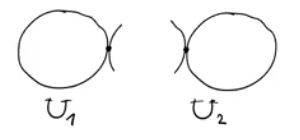
\includegraphics[width=0.4\linewidth]{images/bouquet-circle-fundamental-group}
		\caption{}
		\label{fig:bouquet-circle-fundamental-group}
	\end{figure}
	Possiamo usare il teorema dei CW-complessi per ritrarre $U \sim \Circ^1$ e $V \sim \Circ^1$, mentre l'intersezione è ritraibile in un punto. Quindi diventa che 
	\begin{equation}
	\begin{aligned}
		\pi_1(\Circ^1 \lor \Circ^1, x_0) \simeq \left\langle \alpha, \beta \mid \varnothing \right\rangle \simeq \Z \ast \Z
	\end{aligned}
	\end{equation}
\end{proof}

\begin{xca}
	Dimostriamo il seguente isomorfismo $\pi_1(T_1, x_0) \simeq \Z^2$
\end{xca}
\begin{proof}
	Prendiamo come suddivisione del toro gli aperti $U_1, U_2$ dove $U_1$ è il toro tolto un punto $Q$, mentre $U_2$ è il toro tolto i lati perimetrici che vengono incollati per costruire il toro (si veda la figura)
	\begin{figure}[h]
		\centering
		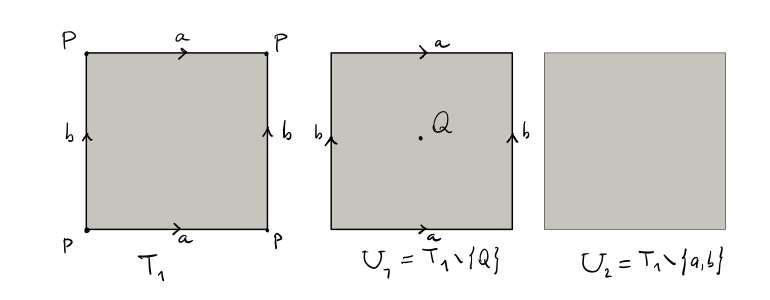
\includegraphics[width=0.7\linewidth]{images/fundamental-group-torus}
		\caption{}
		\label{fig:fundamental-group-torus}
	\end{figure}
	Allora sappiamo che $\pi_1(U_1,x_0) \simeq \pi_1(\Circ^1 \lor \Circ^1, x_0) \simeq \Z \ast \Z$, mentre $U_2$ è contraibile (è essenzialmente un disco aperto). L'intersezione $U_1 \cap U_2$ invece è omotopicamente equivalente a $\Circ^1$, infatti se il buco si può allargare fino ad ottenere $\Circ^1$. Per cui otteniamo i seguenti risultati
	\begin{equation}
	\begin{aligned}
		\pi_1(U_1) & \simeq \Z \ast \Z \\
		\pi_1(U_2) & \simeq \Z_1 \\
		\pi_1(U_1 \cap U_2) &\simeq \Z \\
	\end{aligned}
	\end{equation}
	poiché $\pi_1(U_1 \cap U_2)$ non è banale dobbiamo vedere quale è la relazione $R_{U_1 \cap U_2}$. Per vedere come interagisce sui cappi, dobbiamo ossservare che ogni cappio $c \in \pi_1(U_1 \cap U_2)$ può essere portato sul bordo di $U_1$ e, ciascuno dei cappi $c$ percorre i lati del toro in senso $aba^{-1}b^{-1}$, questo coincide alla relazione sui cappi di $\pi_1(U_1)$: $a \ast b \ast a^{-1} \ast b^{-1} = 1$ (si veda figura)
	\begin{figure}[h]
		\centering
		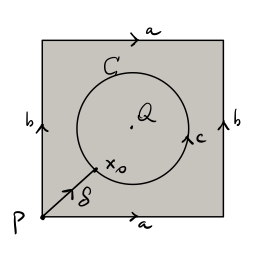
\includegraphics[width=0.4\linewidth]{images/fundamental-group-torus-2}
		\caption{}
		\label{fig:fundamental-group-torus-2}
	\end{figure}	
	per cui diventa
	\begin{equation}
	\begin{aligned}
		\pi_1(U_1 \cup U_2, x_0) \simeq \left\langle \{\alpha, \beta\} \cup \varnothing \mid R_{U_1 \cap U_2} \right\rangle \simeq \left\langle \alpha, \beta \mid \alpha \beta = \beta \alpha \right\rangle \simeq \Z^2
	\end{aligned}
	\end{equation} 
\end{proof}

\begin{xca}
	Dimostrare per ragionamento analogo a quello del toro che 
	
	\begin{equation}
	\begin{aligned}
	\pi_1(U_h, x_0) \simeq \left\langle \alpha_1, \dots, \alpha_h \mid \alpha^2_1 \cdots \alpha^2_h = 1\right\rangle
	\end{aligned}
	\end{equation}.
\end{xca}

